\documentclass[oneside]{tudelft-report}
\newcommand{\comment}[1]{}
\usepackage{enumitem}
\usepackage[acronym,nomain]{glossaries} % Load the glossary pacakage with the acronym option
\setlength{\parskip}{1em}
\usepackage[justification=centering]{caption}
\usepackage{pdfpages}
\usepackage{subcaption}

\newcommand{\noop}[1]{} % a do-nothing command that serves a purpose

\begin{document}

%% Use Roman numerals for the page numbers of the title pages and table of
%% contents.
\frontmatter

\title[Final report\\TI3806 - Bachelorproject]{BEPStore}
\author{Bart Heemskerk}{Wouter Kooyman van Guldener}{Steffan Sluis}
\affiliation{Technische Universiteit Delft}
\coverimage{cover2.jpg}
\makecover

%% Include an optional title page.
\begin{titlepage}

\begin{center}

%% Insert the TU Delft logo at the bottom of the page.
\begin{tikzpicture}[remember picture,overlay]
    \node at (current page.south)[anchor=south,inner sep=0pt]{
        
\includegraphics{cover/logo}
    };
\end{tikzpicture}

%% Extra whitespace at the top.
\vspace*{2\bigskipamount}

%% Print the title in cyan.
{\makeatletter
\titlestyle\color{tudelft-cyan}\Huge\@title
\makeatother}

%% Print the optional subtitle in black.
{\makeatletter
\ifx\@subtitle\undefined\else
    \bigskip
    \titlefont\titleshape\LARGE\@subtitle
\fi
\makeatother}

\bigskip
\bigskip

by
%door

\bigskip
\bigskip

%% Print the name of the author.
{\makeatletter
\titlefont\Large\bfseries\@author
\makeatother}

\vfill

in partial fulfillment of the requirements for the degree of
%in overeenstemming met de vereisten voor het verkrijgen van de graad van

\bigskip
\bigskip

{\bfseries Bachelor of Science}

in Computer Sciences

\bigskip
\bigskip

at the Delft University of Technology,
%aan de Technische Universiteit Delft,

to be defended publicly on Friday June 17, 2016 at 2:30 PM.
%in het openbaar de verdedigen op dinsdag 1 januari om 10:00 uur.

\vfill

\begin{tabular}{lll}
%% Add additional information here, per faculty requirements, e.g
%    Student number: & 1234567 \\
%    Project duration: & \multicolumn{2}{l}{March 1, 2012 -- January 1, 2013} \\
    Coach: & Dr.\ E.A.\ Hendriks, & TU Delft \\
    Client: & L.\ Starovoitova, & Feedbackfruits\\
    Bachelor project coördinators:
        & M.A.\ Larson, & TU Delft \\
        & Dr.\ ir.\ F.F.J.\ Hermans, & TU Delft \\
        & O.W.\ Visser, & TU Delft
\end{tabular}

%% Only include the following lines if confidentiality is applicable.
\bigskip
\bigskip
%\emph{This thesis is confidential and cannot be made public until December 31, 2013.}
%\emph{Op dit verslag is geheimhouding van toepassing tot en met 31 december 2013.}

\bigskip
\bigskip
An electronic version of this thesis is available at \url{http://repository.tudelft.nl/}.
%Een elektronische versie van dit verslag is beschikbaar op \url{http://repository.tudelft.nl/}.

\end{center}

\end{titlepage}



% Define any acronyms
% Use acronyms with the \gls{} or \Gls{} command
\newacronym{rtc}{RTC}{realtime-clock}
\newacronym{adc}{DAC}{digital-to-analog converter}
\newacronym{dac}{ADC}{analog-to-digital converter}
\newacronym[plural=LEDs,firstplural=light emitting diodes (LEDs)]{led}{LED}{light emitting diode}
\newacronym{spi}{SPI}{serial peripheral interface}
\newacronym{i2c}{I$^2$C}{inter-integrated circuit}
\newacronym{pwm}{PWM}{pulse-width modulation}
\newacronym{tx}{Tx}{transceiver}
\newacronym{rx}{Rx}{receiver}
\newacronym{pwb}{PWB}{printed wiring board}
\newacronym{pcb}{PCB}{printed circuit board}
\newacronym{uml}{UML}{unified modelling language}
\newacronym{mvp}{MVP}{minimum viable product}
\newacronym{sig}{SIG}{Software Improvement Group}
\newacronym{ci}{CI}{Continuous integration}

\chapter*{Preface}
\setheader{Preface}

FeedbackFruits is a company that offers an online learning solution to help innovate education. Their platform is used on a daily basis by teachers and students to improve their learning experience. When using the platform, the users often think of valuable feedback and new features they would like to see added. This report describes the process of designing and implementing a platform for the purpose of collecting this feedback in a central location and streamlining the process of acting upon it.

\begin{flushright}
{\makeatletter\itshape
    \@author \\
    Delft, June 2016
\makeatother}
\end{flushright}


\chapter*{Summary}
\setheader{Summary}


\tableofcontents

% reset acronyms
\glsresetall

%% Use Arabic numerals for the page numbers of the chapters.
\mainmatter

% Steffan
\chapter{Introduction}

Albert Einstein once said: "Education is what remains after one has forgotten what one has learned in school." His opinion about education doesn't differ much from the opinion most students have nowadays. FeedbackFruits aims to change this view of education by using modern technology to bring students and teachers together. Although the solution FeedbackFruits provides may solve (part of) the problem, the field of education and the methodologies and technologies around it constantly change. This results in a growing demand for new tools from the consumers of the FeedbackFruits platform and as such the need for software developers to meet this demand.

Here a problem arises: most consumers of the platform are not developers and most developers are not consumers of the platform and as such, the increasingly difficult task of finding developers to meet the demand for new tools falls on FeedbackFruits. In order to simplify this task, the demand for a new 

% Steffan
\section{Context}

% Steffan
\section{Vision}

% Steffan
\section{Potential impact}
% Steffan
\chapter{Client}
The client is FeedbackFruits, a ... company

% Steffan
\section{Needs}

% Steffan
\section{Motivation}
\chapter{Problem}

This chapter gives a description of the problem that was solved over the course of this project. It is divided into two sections. The first section describes the problem that was addressed during this project and the third section gives an analysis of how this problem can be decomposed into smaller problems.

% Wotuer
\section{Problem definition}
In the research report{ref:research-report:v1} a problem description was identified: ``How can the existing platform be extended in such a way that everyone in the FeedbackFruits community can contribute to the software development process?''.

%Wouter
\section{Problem analysis}
The most important aspects to this problem were identified in the research report as being: hype, requirements engineering, code and process updates. 


%Wouter
\chapter{Process}

This chapter describes the specifics of the process followed over the course of this project. It is divided into three sections that each address a vital part of a healthy process. The first section discusses the communication used, while the second section covers how the progress is maintained. The final section addresses how the quality of the code-base is assured.

\section{Communication}
Communication is the most important aspect of the development process as identified in the research report (appendix \ref{app:research_report}). The team works on location, thus verbal communication is the primary method of communication. Slack is used for sharing information that is verbally difficult to share such as links and documents. For communication about code GitHub Pull Requests are used.

%Steffan
\section{Solution requirements}
At the start of the project, two weeks of extensive research were conducted on the subject of collaborative software development and community engagement. To assure a correct solution corresponding to the results found in the research report, the team had a brainstorm session with the purpose of translating the conclusions of the research into a conceptual solution. The result of this session is included in appendix  \ref{app:brainstorm1}. This conceptual solution was then analysed and decomposed into solution requirements (see chapter 6 of the research report).

\section{Progress maintenance}
Progress is mainly protected with a scrum approach. A Waffle.io\footnote{\url{https://waffle.io}} scrum board is used that integrates with GitHub issues and milestones. Furthermore, the teams takes part in the weekly Tuesday meetings at FeedbackFruits. These are feedback sessions in which progress is reported and the whole FeedbackFruits team can comment and give feedback. Besides these weekly meetings, the team meets roughly every two weeks with a representative from FeedbackFruits and Emile Hendriks, the TU Delft coach.

\section{Quality assurance}
The software development process is extensively backed with tools to automatically measure the quality of the project with help of \gls{ci}. Quality can be quantified into many different aspects. \Gls{sig} chose six key properties as key metrics: volume, redundancy, unit size, complexity, unit interface size and coupling \Citep{sig2012}. Furthermore, tools are used to improve the code-style and the stability of the platform.

\subsection{Code climate}
To improve the maintainability of the code, CodeClimate\footnote{\url{https://codeclimate.com}} is used. CodeClimate assesses and advises on the complexity, duplication, security and style of the code. Besides CodeClimate, tools such as Rubocop\footnote{\url{http://batsov.com/rubocop/}} and JSHint\footnote{\url{http://jshint.com/}} are used for more specific complexity and style improvements. The aim is to have the maximum CodeClimate score of $4.0$ and have no Rubocop and JSHint errors.

\subsection{High cohesion, loose coupling}
Smaller systems are easier to understand and maintain. Although the proposed system will not be very high in volume, it may get bulky when a lot of features are implemented. To overcome this issue, the system is decomposed into separate components that are each responsible for a specific functionality. This makes adding features to the system relatively easy and reduces the risk of breaking the system.

\subsection{Continuous integration}
To maintain a stable production environment of a high quality, \gls{ci} by CircleCI\footnote{\url{https://circleci.com}} is used. CircleCI takes care of automatically building and running the tests when a commit is pushed to GitHub.

\subsection{Testing}
While testing should not be a goal in itself, it is a useful asset to verify whether the system does what it is supposed to do. To automatically measure how much of the code the tests cover, Codecov\footnote{\url{https://codecov.io}} is used as a GitHub integration. The aim is to continuously have a code-coverage of above $90\%$.


% Most These tools are GitHub pull-requests, CircleCIn the list below, the used tools are listed and described. 

% \begin{description}[align=right,labelwidth=3cm]
%     \item [GitHub] pull requests are used to discuss and improve the code before it is merged into the main codebase;
%     \item [CircleCI] continuous integration, utilising the RSpec test suite and Rubocop for style;
%     \item [CodeCov] test coverage;
%     \item [CodeClimate] 
% \end{description}

% CircleCI is configured to 

\chapter{Solution}

This chapter explains how the solution works for the problem that was described in Chapter 1. It is divided into two sections. The first section gives a formal specification of the solution. The second section shows how this formal specification was implemented over the course of this project.

%Bart
\section{Specification}
It appears that GitHub already implements most of the features needed as specified in the problem analysis. The resulting platform should therefor be an extension to the GitHub platform so it can also be used by non-developers. In the research report a MoSCoW model was proposed \Citep * [chap. 5.5]{research-report:v1.0}

\subsection{Requirements}
MoSCoW

\subsection{Success critera/Use Cases}
% Maybe split this into formal/informal?

\subsection{Definition of Done}
Iets over ons eigen platform gebruiken om zichzelf te ontwikkelen.


\section{Implementation}
% issue 11
Complete description of the final product. %plus graphics

% FlowChart

% UML Diagram

% Plaatje van uiteindelijke platform (?)


% \section{Conclusion}

\chapter{Conclusion}

Over the course of this project, several problems were addressed and solutions were found. This chapter analyses the solution in order to show how and to what extent it solves the problems. The chapter is divided into three sections. The first section draws conclusions about the results of the comparison between the solution and its implementation. The second section gives recommendations for building upon the implemented solution. The third section suggests how the research done for this project might be expanded upon.

\section{Results}

The previous chapter compares the implemented solution with the requirements found during the research phase of the project. In this comparison, the most remarkable differences can be found in the coverage of the different use case that were specified. Of the four use cases, the third and fourth use case could not be fulfilled with the current solution implementation. These use cases are concerned with the share of designs and giving feedback on community contributions. These features were not implemented due to a revision of the planning because of delays.

Looking at the solution requirements it becomes clear that the solution mostly lacks a feedback system. This will have impact on the engagement of the users, because feedback promotes engagement. The reason that these requirements were not fulfilled during the development is also due to the revision of the planning. In the implementation, the issues and milestones are displayed, therefore giving feedback on the process of the goal. To get feedback on the quality of the goal and the work of an individual, the solution must request information about the content of contributions. Doing that in an effective way turned out to be more complicated then originally estimated. GitHub facilitates the feedback in a proper way for the developers, the main users of the feedback. Because of that, it was decided that the feedback about code and quality should remain on GitHub for this version of the solution.

% Steffan
\section{Recommendations}
The most important recommendation is to implement a feedback mechanism as described in the previous section. Such a mechanism would boost the engagement of the platform and increase the ease of determining the value of community contributions.

Additionally, the implemented solution is designed to accommodate integrations with external services. Due to the scope of the project, 
the amount of available integrations is not very large. If the solution is adopted by the client, it is recommended to implement integrations for other services. The integrations that are implemented with the solution focus on the link between developers and non-developers. Because of this, it would be beneficial to focus on integrations with services that target other parts of the software development process, or aspects around it, such as the design of software components.

Furthermore, the implementation of requirements engineering within the solution could be improved. Currently a small layer of extra functionality is added to GitHub issues and milestones. This process could be extended to integrate these issues and milestones better into the solution.

\section{Further research}
The research that was performed over the course of this project unites community engagement with distributed software development, and aims to provide guidelines towards implementing a platform that unites these subjects. It could possibly be expanded upon by finding guidelines for the union of community engagement in other fields and processing these into a general process for stimulating community engagement.

Alternatively, further research could target the more specific forms of community engagement in software development to offer a comparison of the effectiveness of different techniques. The research on community engagement performed over the course of this project offers general guidelines rather than a specific set of instructions or a particular method.

%% Use letters for the chapter numbers of the appendices.
\appendix

\chapter{Original project description}
This chapter contains the problem description as originally formulated by the client. It is divided into the three orignal sections pertaining to the problem, the company and any auxiliary information.

\section{Project description}
Open source software development has grown during past years. With the adoption of Pull Requests as a means of performing code review and Continuous Integration and Continuous Deployment, an interesting model for software development has arisen: crowd-sourced software development.

On the other hand, micro-service oriented application structures have also become popular over the last years. This application architecture often allows for new functionalities to be added with little effort and with decreased risk of unintended consequences, since each part of the application as a whole functions independently. If one part breaks, it doesn't necessarily affect others.

The project consist of building a platform that streamlines the process of building a micro-service that can interact with the FeedbackFruits API. The goal is to allow developers to immediately create new functionalities, with little knowledge about the internal workings of the API. The platform should offer a set of requirements for functionalities, which can be tested for automatically, as well as the ability to request new functionalities, given a set of requirements.

The platform is targeted at developers who are not (completely) familiar with the codebase of the application they are expanding. For that reason, the main goal of the platform should be to streamline the process from feature request to pull request.

During the project, students may encounter the following problems:
\begin{itemize}[nosep]
    \item What kinds of requirements can be automatically tested for, and what kinds can't?
    \item How and when should communication work between platform, developer, feature requester and application maintainers?
    \item How and when does a service become deprecated? How is it maintained?
    \item What feature requests have priority over others, and why?
    \item How does my service communicate with others?
\end{itemize}

\section{Company description}

We are a startup improving education for learners worldwide. Our platform is built on modern web technologies like Rails, Ember.js, HTML5 MongoDB, Elasticsearch and Git. With more than 30K users and a team of over 20 professional geeks, we work to make education better! We are very passionate and dedicated to our mission. Our devteam ranges from students who hack on education part time to full time, full stack, experienced coders. If you would like to join us in making student life better one pull request at a time and want to dig deeper into web building while doing so, keep on reading!

Our product owner, design and development teams work closely together. We work agile using short 2-week release cycles. A number of our developers have done their own graduation projects within FeedbackFruits, while studying at TU Delft. They are well familiar with the process and will be able to give you valuable advice and guidance. Our 2.0 platform on which you would be working is modularized, meaning that you will have significant freedom in choosing the technology you would like to use in your project. 

\section{Auxiliary information}

You will be able to work on the project from our office located in the startup incubator Yes!Delft. This will allow you to experience the awesome atmosphere in the startup community and being around some of the most innovative businesses in Europe. You will be renumerated for the work on your project and will enjoy all the awesome free lunches, weekly dinners, and other team events like sailing trips and prison breaking.

Our team consists of both dutch and international people, therefore, you will be able to write your proposal in the preferred by you language (Dutch or English). We do not oppose any limitations as to the group size, but would recommend a group size of 2-3 people. One student (R.S. Sluis) has already confirmed his participation in this project.

Last but not least you will have the opportunity to be coached by Emile Hendriks, the director of Computer Science education at TU Delft. Emile has published over 100 papers in international journals and conferences and has supervised over 50 master students and co-supervised 10 PhD students and is one of the leading educational visionaries in the Netehrlands. .
\chapter{Solution Requirements}\label{app:solution_req}

In the initial research report\footnote{\url{https://bep-store.gitbooks.io/research-report/content/v/f60f68494dba238334cb22dc076b64b55bbae851/}} a MoSCoW model \Citep{moscow2014} was proposed as the requirements for the platform. The following requirements are the proposed requirements, separated by must-have, should-have, could-have and won't-have. 

\section*{A user of the platform must be able to:}
\begin{itemize}[nosep]
    \item See a landing page
    \item create a account
    \item view a list of goals
    \item create a goal
    \item join a goal as core team member
    \item see a goals description
    \item see a list of (sub-)challenges for a goal
    \item prioritise (sub-)challenges
    \item use GitHub integrated
    \item decompose a goal into (sub-)challenges in a structured way \Citep {hoffmann2004requirements}
    \item get the following information about a goal:
        \begin{itemize}
            \item progress
            \item milestones/challenges
            \item quality
        \end{itemize}
    \item get feedback on his/her work (via peer review)
    \item give feedback on the work of another user
    \item communicate with other users
\end{itemize}
\section*{A user of the platform should be able to:}
\begin{itemize}[nosep]
    \item have a general information page
    \item join a goal as a contributor
    \item set estimated necessary resources for a goal
    \item set estimated necessary tags for a goal
    \item edit a goal he/she owns
    \item view a list of newest goals
    \item search/browse for goals
    \item hype his/her goals by sharing it on social media
    \item get the following information about a goal:
        \begin{itemize}
            \item a timeline
            \item the functionality
        \end{itemize}
    \item get feedback on his/her work via automated testing
    \item communicate with other users via different tools 
    \item get updates via push-notifications, e-mail etc.
    \item see his/her contributions
\end{itemize}
\section*{A user of the platform could be able to:}
\begin{itemize}[nosep]
    \item edit his/her account
    \item be able to join a project as a backer
    \item view a list of trending goals
    \item get the following information about a goal:
        \begin{itemize}
            \item bounty
            \item availible resources
            \item hype factor
        \end{itemize}
    \item get reputation
    \item view the reputation of a user
    \item be engaged through gamification
    \item follow a tutorial on how to use the platform
    \item get tips on how to use the platform
\end{itemize}
\section*{A user of the platform won't be able to:}
\begin{itemize}[nosep]
    \item follow a tutorial on how to use the platform, based on the type of user
    \item join a training party
    \item take part in a ranking system
    \item be matched with an apprentice
    \item be matched with a senior
\end{itemize}
\chapter{Infosheet}
\chapter{Research Report}\label{app:research_report}

This chapter includes the final version of the research report. It describes the problem that was solved during this project, the research questions associated with this problem and the conclusions to these questions based on the research that was performed. It should be noted that section 5.5 of the research report contains a revised version of the solution requirements. The orignal version of the solution requirements is included in appendix B.


\includepdf[pages=-]{./media/research-report.pdf}
\chapter{Conceptual Solution}\label{app:brainstorm1}
Figure \ref{fig:brainstorm} shows the results of the most important brainstorm session at the start of the project.
\begin{figure}[ht]
    \centering
    \includegraphics*[width=\textwidth]{./media/brainstorm}
    \caption{Result of the most important brainstorm session}
    \label{fig:brainstorm}
\end{figure}


\chapter{\texorpdfstring{\Gls{sig}}{SIG} Feedback}
There are two checks performed by \gls{sig}. The feedback for the first check was in Dutch and has been translated. The results for the second check have not yet been received so could not be processed.

\section{Feedback content}
The code of the system scores 4.5 stars on our maintainability-scale, which means that the maintainability of the code is above average. However, improvements can be made when it comes to duplication.

Duplication is determined by looking at the percentage of code which is redundant, primarily the code that has multiple occurrences in the system and can be removed. From the perspective of maintainability, it is desirable to have a low percentage of redundancy, because adjustments to the redundant code have to be done in multiple places.

Multiple duplications are found in the code. For example, the file \textit{click-outside.js} is present two times in the implementation. Duplication was found between the files \textit{show.js}, \textit{edit.js} and \textit{deploy.js}. In the html-code (\textit{422.html}, \textit{404.html} and \textit{500.html}) duplication also occured. The same 45 lines of code are present in all three locations. Try to rewrite the code in a easier way, such that the code can be reused instead of duplicated.

Finally it is good to see that you have written a lot of test-code besides the production-code. The ratio of test-code and production-code is 2:3.

We hope that you are able to maintain the quality of the code as well as the ratio of test-code and production-code during the remainder of the project.''

\subsection{Processing of feedback}
The feedback indicates that the structure of the implementation is good. \Gls{sig} is satisfied with the ratio of test-code and production-code. Combined with the test coverage aggregated by CodeCov, the end-product will be well-tested.

The only negative comments are about code duplications. While the duplication in the html-code were auto-generated by \textit{Ruby on Rails}, they were corrected nonetheless.

The other duplications were in the files \textit{show.js}, \textit{edit.js} and \textit{deploy.js}. However, after investigation it was concluded that \textit{deploy.js} was misspelled and should actually have been \textit{destroy.js}. To remove most of the duplication, the recurring parts were combined into its own function. Part of the duplication is caused by simple import statements. It does not make sense to refactor those.

\subsection{After the feedback}
After the feedback was received, the team was more keen on spotting and avoiding code duplication in (each others) pull requests. Pull requests were only merged if the duplication was removed. According to CodeClimate the \textit{Rails-api} has no duplications at all, and the \textit{Ember-ui} indicates that there are two small duplications. The fixes for these duplications make the code less readable, so it has been decided to not remove those duplications.

% De code van het systeem scoort 4.5 ster op ons onderhoudbaarheidsmodel, wat betekent dat de code bovengemiddeld onderhoudbaar is. Er zijn echter een paar verbeteringspunten bij Duplication.

% Voor Duplicatie wordt er gekeken naar het percentage van de code welke redundant is, oftewel de code die meerdere keren in het systeem voorkomt en in principe verwijderd zou kunnen worden. Vanuit het oogpunt van onderhoudbaarheid is het wenselijk om een laag percentage redundantie te hebben omdat aanpassingen aan deze stukken code doorgaans op meerdere plaatsen moet gebeuren. 

% Er zijn in dit project meerdere duplciaties te vinden: bijvoorbeeld het click-outside.js bestand is twee keer in de upload aanwezig. Verder is duplicatie gevonden tussen de bestanden show.js, edit.js en deploy.js. Ook in de html code (422.html 404.html, 500.html) is de code gekopieerd, dezelfde 45 lines of code zijn aanwezig op alle drie verschillende locaties. Probeer deze code te herschrijven op een slimmere manier, zodat de code wordt hergebruikt in plaats van gedupliceerd. 

% Tot slot is het goed om te zien dat jullie naast productiecode ook redelijk veel testcode hebben geschreven. De verhouding tussen testcode en productiecode is 2:3. 

% Hopelijk lukt het jullie nog om zowel de kwaliteit van de code als de verhouding tussen testcode en productiecode tijdens het vervolg van het project te behouden.
\chapter{Reflection}
This chapter presents the reflection of the team of on the projects. It is divided into three sections. The first section is about the problems that were presented during the process of solving the problem. Section two describes the particular challenges of finding a solution to the problem. The third section presents the personal reflections by each of the team members.

\section{Process}
During the process of implementing a solution to the problem, the biggest problem proved to be planning. Although planning and process management have been a point of attention from the start of the project, the biggest challenge turned out to be correctly assessing the amount of time needed to implement features. During the weekly scrum meetings, it often turned out that some features were more complex than previously assessed, resulting in delays during that iteration that were carried over to the next iteration.

A simple solution to the problem described above might be to simple move on from delayed features and deal with the next iteration as a separate concern. However, in software development this is not always possible since future functionalities might depends on features from the current iteration. Another solution might be to revise the planning once a delay occurs. This solution was applied by the team, and although the implemented solution did not adhere to every requirement, the result did satisfy the most important requirements.

\section{Solution}
The solution found as a result of the research can be applied in other contexts than that of the client. In addition, the research presented findings that the team found personally interesting. This resulted in the team being more engaged in the subject and the project. This was emphasised by the educational context of the problem and its relation to software development. With regards to the implemented solution, the team would have like to do more. Although it can be expected that a planning might change, the team became invested in the project, often placing personal plans second to put the project first. 

\section{Challenges}
In implementing the solution, the team tried to follow the philosophy and architecture behind the client's platform. In doing so, they were presented with a few challenges. For some of the team members, understanding the architecture of the client's platform proved difficult at first due to the fragmented nature of the platform. To other team members, a lack of experience in commercial software development was a barrier to overcome. However, due to the support of other team members and the general collaborative effort between team members, these problems were overcome over the course of the project.

\section{Personal reflection}
The following sections describe the personal reflection of the team members of this project. It is written from a first person perspective. The contents of the reflection represent several aspects of the project, ranging from prior knowledge to satisfaction with the implemented solution.

\subsection{Bart Heemskerk}
At the start of the project I had no experience with either Ember or Ruby, so I had a lot of catching up to do in order to understand the platform of the client, let alone build an application using the styles already provided by the client. Part of the application was planned to be integrated in the platform of the client, which was a basis as well as a restriction. When the actual coding started, I started creating the basis of the user interface en practically never left.

Designing and implementing the user interface was a new experience because I used to create the code which gave the user interface its functionality without bothering much how the application worked. Having the styles from the client helped me create a basis, after which we could create our solution as we intended to. Thanks to the rest of the team I was quickly able to implement every component in a rapid pace. I am thankful for the patient for the patient they had when I had another question.

Although the solution lacks some of the intended functionalities, I think that the solution can fulfil its intended purpose. The solution enables the users of the platform of the client to address the lack of a certain functionality, feedback that is valuable for the client. The solution also facilitates that the functionality can be created without the help of the client. Because the solution implements the elements that GitHub lacks and are needed for the development of the micro-services, I think that the solution is an addition to the platform of the client. Therefor I can say that I am proud of what we have created.

\subsection{Wouter Kooyman van Guldener}
Let me start by saying that I enjoyed this project very much. Especially the environment at FeedbackFruits was very inspiring and has helped keeping our motivation high. Also, the fact that we kept everything (even all the reports) open-source stimulates to deliver quality work.

Personally, I think the cooperation with Bart and Steffan went very well, we really complemented each other. Steffan was already familiar with the existing platform and frameworks and could help Bart and me out in several occasions. Bart was really excelling with his design skills. While we all had our own expertise, the use of pull-requests really helped to keep everyone sharp and involved in every aspect of the project.

Improvements to the process could be made though, especially in keeping the planning up to date. It frequently occurred that we were too optimistic in our planning and did not meet the set requirements for a milestone. A solution to this could be to adhere more to the Scrum methodology and assign weights and time indications to each and every issue in the backlog. On the other hand, having a too optimistic planning may not be a bad thing. If you do not get demotivated if you do not meet the planning, it may stimulate someone to work harder to actually meet the target.

Another improvement could be made in the update rounds with Emile Hendriks, our coach. I feel that the the meetings could have been better prepared with respect to showing what we actually did the past period. This does not apply to updating the client because of the Tuesday-evening update rounds at FeedbackFruits.

\subsection{Steffan Sluis}
I had been an employee of the client for over a year at the start of the project. I was closely involved with the inception of the project, which resulted in me acting as a bridge between the client and the team. It also meant the barrier of understanding the subject and the context of the project was substantially lower for me. At the start of the project, this resulted in a lot of collaborative work between me and the rest of team. This changed quickly after starting the implementation phase of the project, since the team picked up on the client's platform architecture very quickly.

The solution that was implemented does not cover all of the intended requirements. In my opinion, the scope of the research and extensibility of the solution more than compensates for this. The target of the project has always been to facilitate the involvement of others in the improvement of software, and the implemented solution reflects the focus on inclusion and extensibility rather than the implementation of particular features. I am happy with the results.

\chapter{Design and implementation}

This chapter compares the designs that were made over the course of the project to that of the solution implementation. The designs that are compared are that of the goals, issues and chat. These cover the most important aspects of the platform: collaborative innovation, problem decomposition and communication.

\section{Goals}

\begin{figure}[ht!]
    \centering
    \begin{subfigure}[b]{0.45\textwidth}
        \includegraphics[height=\textwidth, angle=90]{./media/goal_design}
        \caption{The design for viewing a single goal}
        \label{fig:goal-design}
    \end{subfigure}
    ~ %add desired spacing between images, e. g. ~, \quad, \qquad, \hfill etc. 
      %(or a blank line to force the subfigure onto a new line)
    \begin{subfigure}[b]{0.45\textwidth}
        \centering
        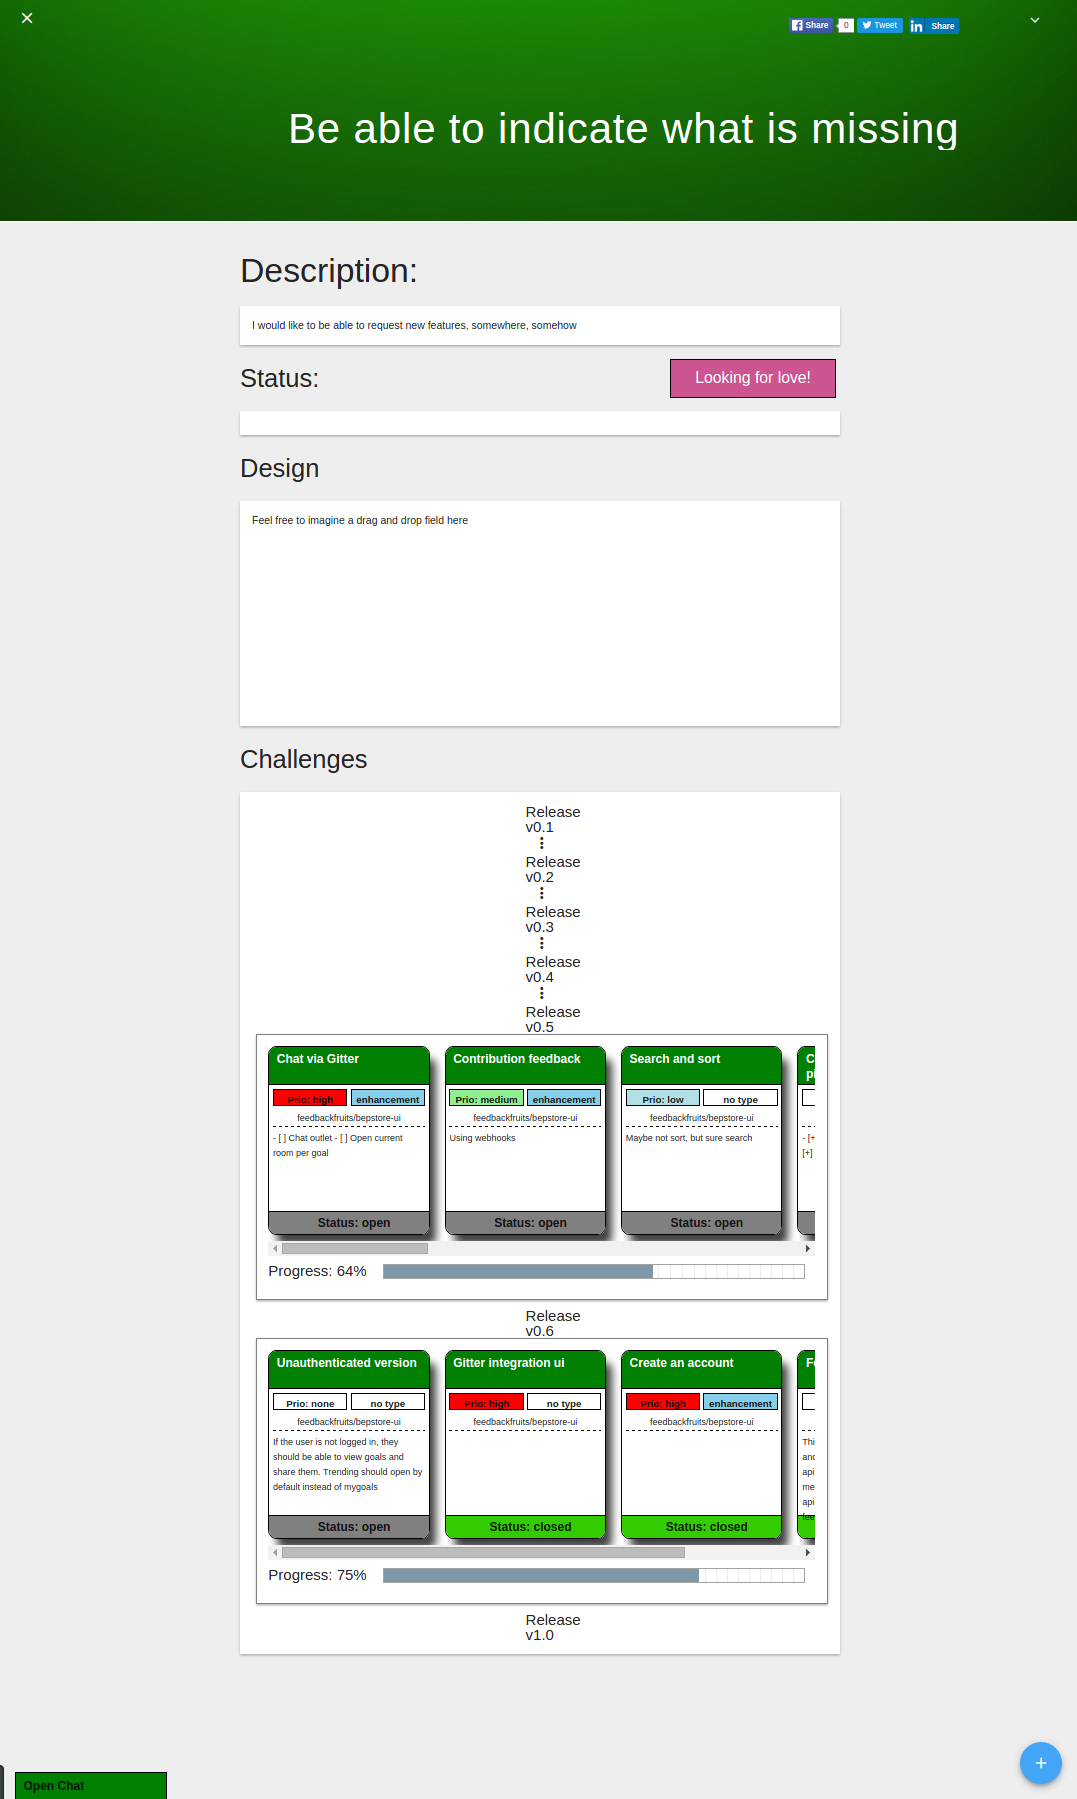
\includegraphics[width=\textwidth, height=0.45\textheight, keepaspectratio]{./media/goal_implementation}
        \caption{The implementation for viewing a single goal}
        \label{fig:goal-implementation}
    \end{subfigure}
\end{figure}
\clearpage
\section{Issues}

\begin{figure}[ht!]
    \centering
    \begin{subfigure}[b]{0.45\textwidth}
        \centering
        \includegraphics[height=0.75\textwidth, angle=90]{./media/issue_design}
        \caption{The design for viewing a single issue}
        \label{fig:issue-design}
    \end{subfigure}
    ~
    \begin{subfigure}[b]{0.45\textwidth}
        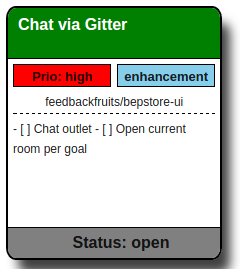
\includegraphics[width=\textwidth]{./media/issue_implementation}
        \caption{The implementation for viewing a single issue}
        \label{fig:issue-implementation}
    \end{subfigure}
\end{figure}

\section{Chat}

\begin{figure}[ht!]
    \centering
    \begin{subfigure}[b]{0.45\textwidth}
        \centering
        \includegraphics[height=0.75\textwidth, angle=90]{./media/chat_design}
        \caption{The design for viewing the chat}
        \label{fig:chat-design}
    \end{subfigure}
    ~
    \begin{subfigure}[b]{0.45\textwidth}
        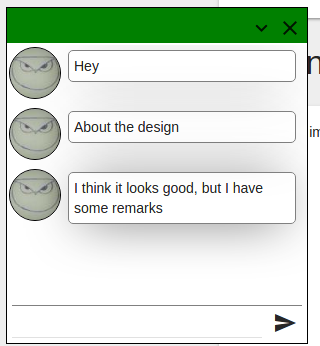
\includegraphics[width=\textwidth]{./media/chat_implementation}
        \caption{The implementation for viewing the chat}
        \label{fig:chat-implementation}
    \end{subfigure}
\end{figure}


\bibliography{report}

\end{document}

